% VLDB template version of 2020-08-03 enhances the ACM template, version 1.7.0:
% https://www.acm.org/publications/proceedings-template
% The ACM Latex guide provides further information about the ACM template

\documentclass[sigconf, nonacm]{acmart}
\usepackage{graphicx} % Required for inserting images
\usepackage{amsmath}
\usepackage{mathtools}
% \usepackage[margin=1cm]{geometry}


\begin{document}
\title{CogSci 131: Back Propagation Assignment}

\author{Chanwut (Mick) Kittivorawong (SSID: 3037251249)}

\begin{teaserfigure}
    \centering
    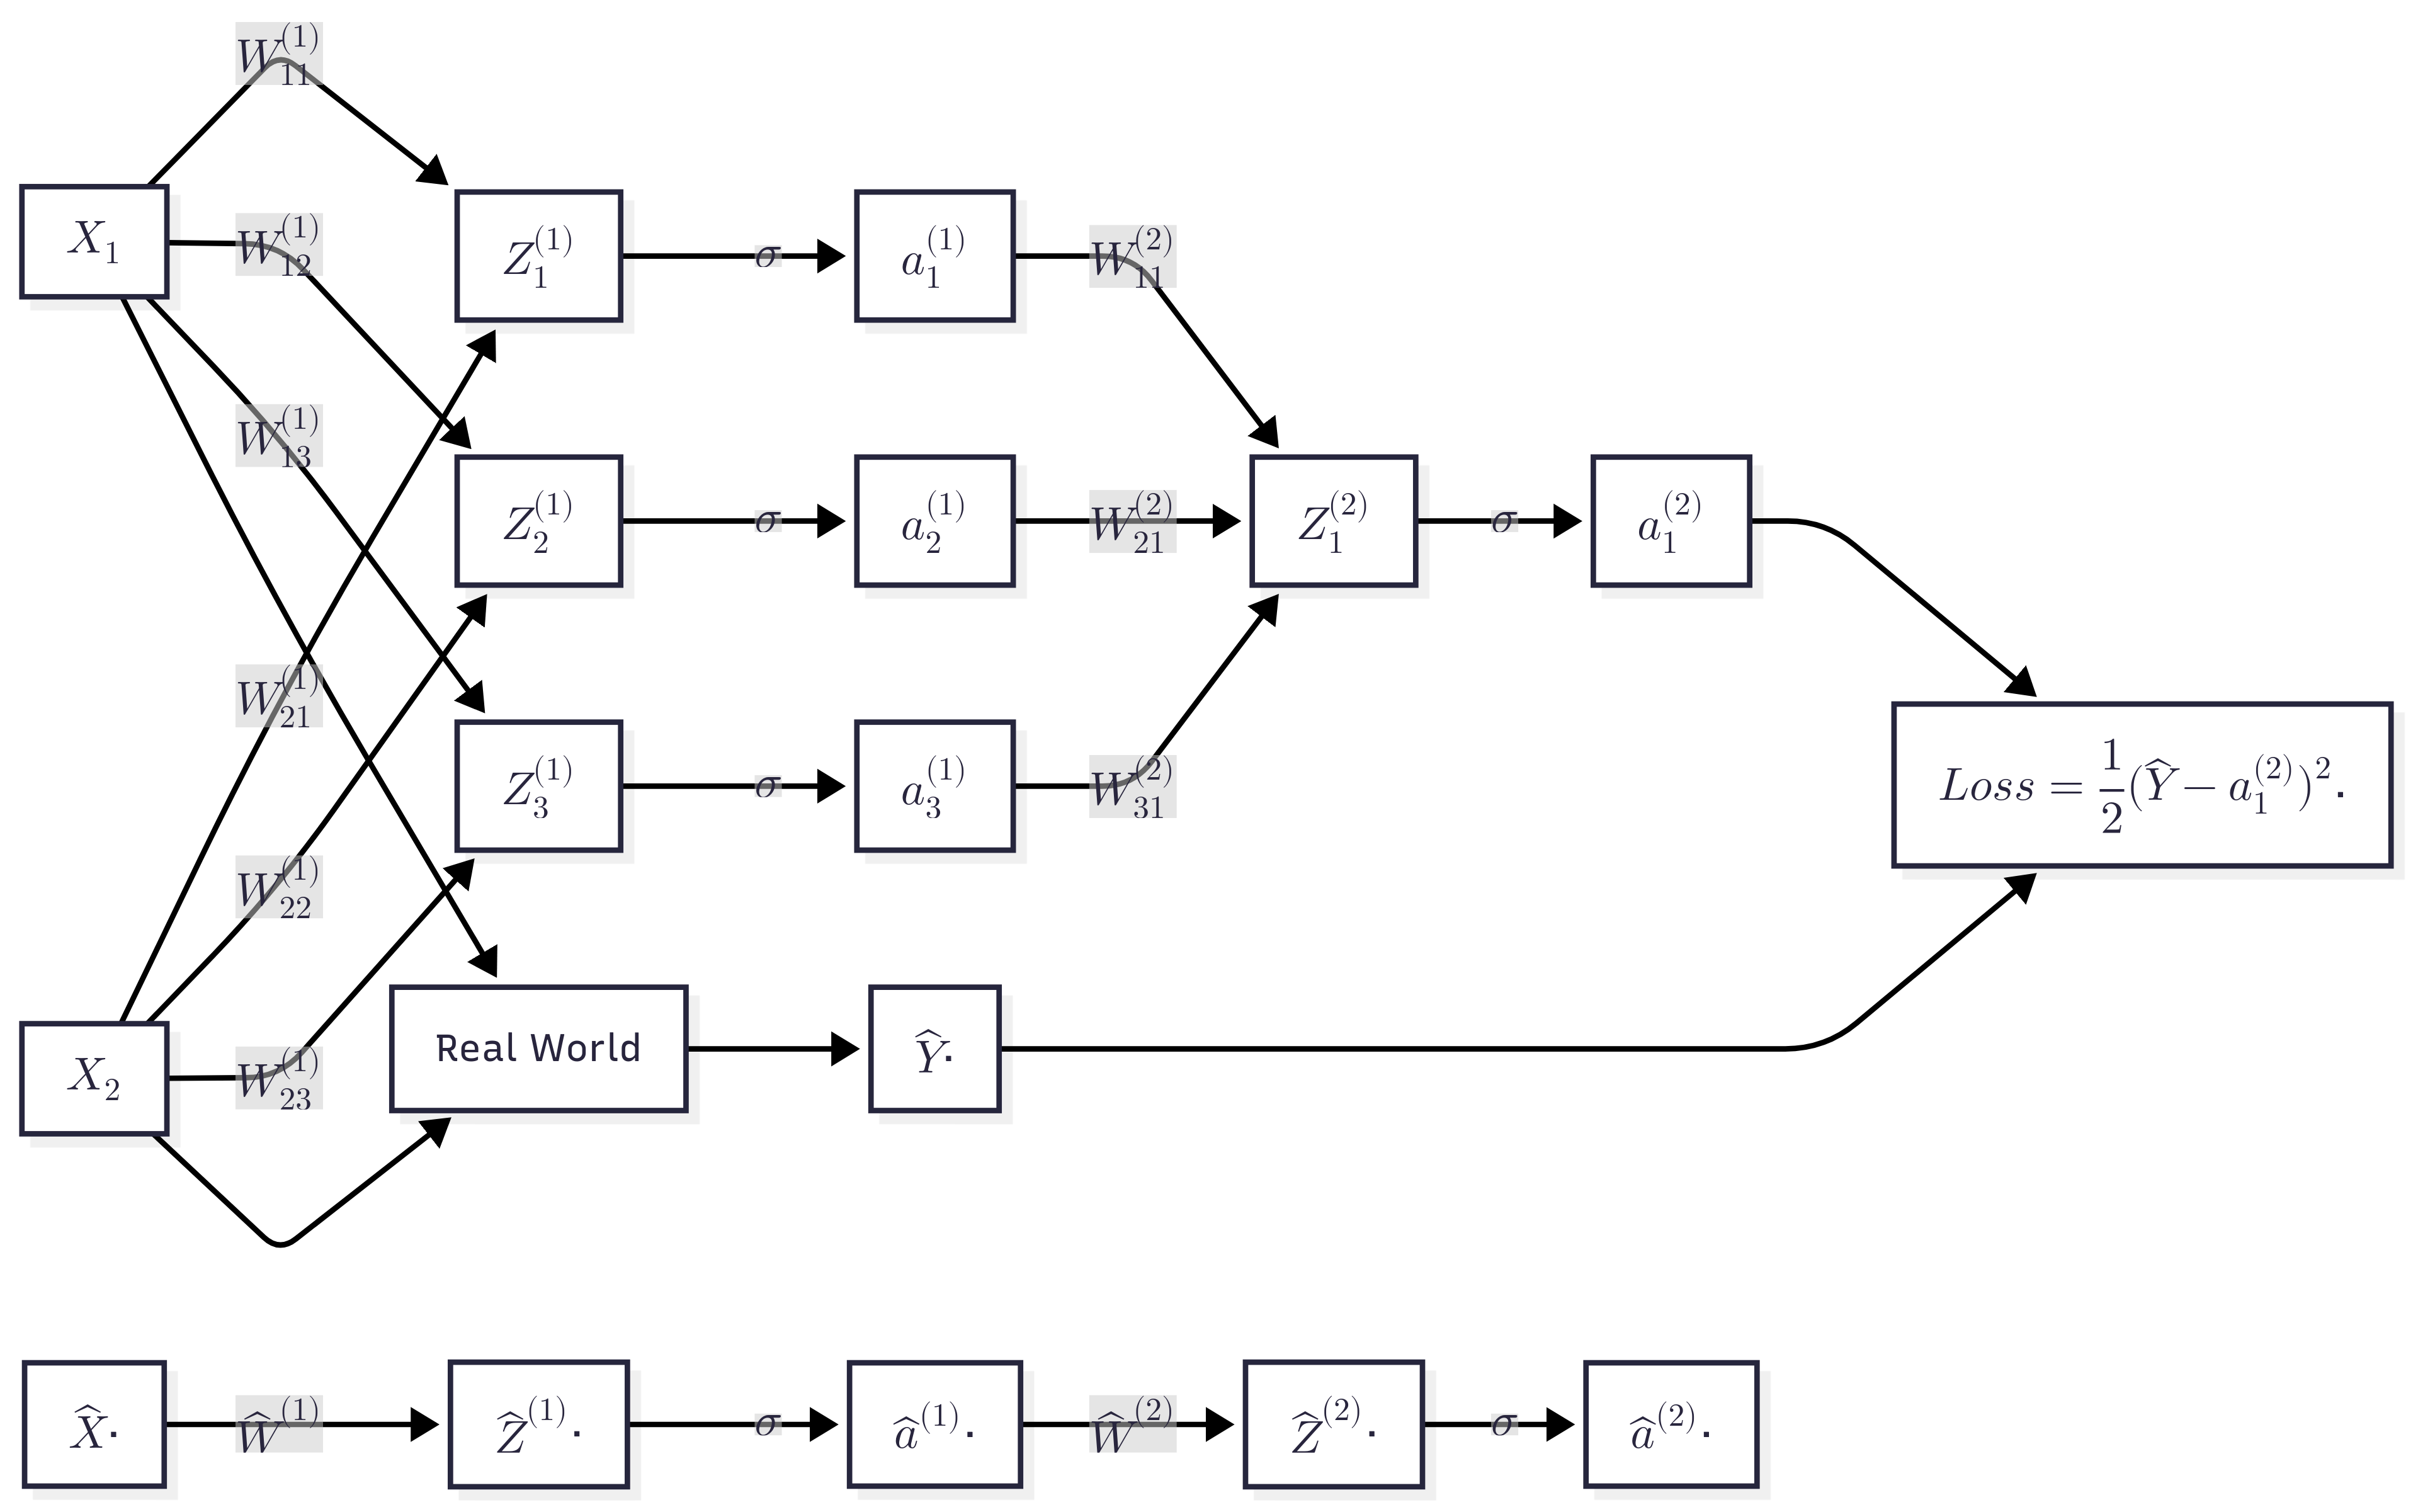
\includegraphics[width=\textwidth]{nn.png}
  \caption{Neural Network Diagram.}
  \Description{Neural Network Diagram.}
\end{teaserfigure}

\maketitle

\section{All variables}
Below are all the variables in the neural networks.

\newcommand{\X}{$\hat{X} = \begin{bmatrix}
X_1 &
X_2
\end{bmatrix}$}
\newcommand{\WOne}{
$\hat{W}^{(1)} = \begin{bmatrix}
W^{(1)}_{11} & W^{(1)}_{12} & W^{(1)}_{13}\\
W^{(1)}_{21} & W^{(1)}_{22} & W^{(1)}_{23}
\end{bmatrix}$
}
\newcommand{\ZOne}{
$\hat{Z}^{(2)} = \begin{bmatrix}
Z^{(2)}_1 &
Z^{(2)}_2 &
Z^{(2)}_3
\end{bmatrix}$
}
\newcommand{\aOne}{
$\hat{a}^{(2)} = \begin{bmatrix}
a^{(2)}_1 &
a^{(2)}_2 &
a^{(2)}_3
\end{bmatrix}$
}
\newcommand{\WTwo}{
$\hat{W}^{(2)} = \begin{bmatrix}
W^{(2)}_{11} &
W^{(2)}_{21} &
W^{(2)}_{31}
\end{bmatrix}^\top$
}
\newcommand{\ZTwo}{
$\hat{Z}^{(3)} = \begin{bmatrix}
Z^{(3)}_1
\end{bmatrix}$
}
\newcommand{\aTwo}{
$\hat{a}^{(3)} = \begin{bmatrix}
a^{(3)}_1
\end{bmatrix}$
}
\newcommand{\Loss}{
$L = \tfrac{1}{2} (\hat{Y} - a^{(3)}_1)^2$
}


\begin{tabular}[h]{l l}
{\WOne} & {\X} \\
{\ZOne} & {\ZTwo} \\
{\aOne} & {\aTwo} \\
{\WTwo} & {\Loss}
\end{tabular}
\section{Forward Propagation}
\subsection{Layer 1}

\subsubsection{Calculating $\hat{Z}^{(2)}$}
Given $\hat{Z}^{(2)} = \hat{X} \times \hat{W}^{(1)}$\\
Then, $\begin{bmatrix}
Z^{(2)}_1 &
Z^{(2)}_2 &
Z^{(2)}_3
\end{bmatrix} = \begin{bmatrix}
X_1 &
X_2
\end{bmatrix} \times \begin{bmatrix}
W^{(1)}_{11} & W^{(1)}_{12} & W^{(1)}_{13}\\
W^{(1)}_{21} & W^{(1)}_{22} & W^{(1)}_{23}
\end{bmatrix}$\\
Then,
$Z^{(2)}_{i} = \sum_{j=1}^{j \le 2} X_j W^{(1)}_{ji}$

\subsubsection{Calculating $\hat{a}^{(2)}$}
Given $\hat{a}^{(2)} = \sigma(\hat{Z}^{(2)})$\\
Then,
$a^{(2)}_{i} = \sigma(\sum_{j=1}^{j \le 2} X_j W^{(1)}_{ji})$

\subsection{Layer 2}
\subsubsection{Calculating $\hat{Z}^{(3)}$}
Given $\hat{Z}^{(3)} = \hat{a}^{(2)} \times \hat{W}^{(2)}$\\
Then, $\begin{bmatrix}
Z^{(3)}_1
\end{bmatrix} = \begin{bmatrix}
a^{(2)}_1 &
a^{(2)}_2 &
a^{(2)}_3
\end{bmatrix} \times \begin{bmatrix}
W^{(2)}_{11}&
W^{(2)}_{21}7
W^{(2)}_{31}
\end{bmatrix}^\top$\\
Then,
$Z^{(3)}_{1} = \sum_{i=1}^{i \le 3} a^{(2)}_i W^{(2)}_{i1}$

\subsubsection{Calculating $\hat{a}^{(3)}$}
Given $\hat{a}^{(3)} = \sigma(\hat{Z}^{(3)})$\\
Then,
$a^{(3)}_1 = \sigma(\sum_{i=1}^{i \le 3} a^{(2)}_i W^{(2)}_{i1})$

\subsection{Loss}
\begin{flalign*}
L &= \tfrac{1}{2}(\hat{Y} - \sigma(\sum_{i=1}^{i \le 3} a^{(2)}_i W^{(2)}_{i1}))^2\\
 &= \tfrac{1}{2}(\hat{Y} - \sigma(\sum_{i=1}^{i \le 3} \sigma(\sum_{j=1}^{j \le 2} X_j W^{(1)}_{ji}) W^{(2)}_{i1}))^2
\end{flalign*}


\section{Backward Propagation}
\subsection{Layer 2}
Updating the 2nd layer's weight.
\begin{flalign*}
    \hat{W}^{(2)}_{new} &= \hat{W}^{(2)}_{old} - \tfrac{\partial L}{\partial \hat{W}^{(2)}}
\end{flalign*}

\noindent
Therefore, we are calculating.
\begin{flalign*}
\tfrac{\partial L}{\partial \hat{W}^{(2)}} &= \begin{bmatrix}
    \tfrac{\partial L}{\partial W^{(2)}_{11}} &
    \tfrac{\partial L}{\partial W^{(2)}_{21}} &
    \tfrac{\partial L}{\partial W^{(2)}_{31}}
\end{bmatrix}^\top
\end{flalign*}

\noindent
For all $1 \le i \le 3$:
\begin{flalign*}
    \tfrac{\partial Z^{(3)}_{1}}{\partial W^{(2)}_{i1}}
    &= \tfrac{\partial \sum_{j=1}^{j \le 3} a^{(2)}_j W^{(2)}_{j1}}{\partial W^{(2)}_{i1}}\\
    &= \sum_{j=1}^{j \le 3} \tfrac{\partial a^{(2)}_j W^{(2)}_{j1}}{\partial W^{(2)}_{i1}}\\
    &= \tfrac{\partial a^{(2)}_i W^{(2)}_{i1}}{\partial W^{(2)}_{i1}}
     + \tfrac{\partial a^{(2)}_j W^{(2)}_{j1}}{\partial W^{(2)}_{i1}}
     + \tfrac{\partial a^{(2)}_k W^{(2)}_{k1}}{\partial W^{(2)}_{i1}} & \text{; $i \ne j \ne k$}\\
    &= \tfrac{\partial a^{(2)}_i W^{(2)}_{i1}}{\partial W^{(2)}_{i1}} + 0 + 0\\
    &= a^{(2)}_i & \text{--- (1)}
\end{flalign*}
\begin{flalign*}
    \tfrac{\partial a^{(3)}_{1}}{\partial W^{(2)}_{i1}}
    &= \tfrac{\partial \sigma(Z^{(3)}_{1})}{\partial W^{(2)}_{i1}}\\
    &= \tfrac{\partial \sigma(Z^{(3)}_{1})}{\partial Z^{(3)}_{1}} \tfrac{\partial Z^{(3)}_{1}}{\partial W^{(2)}_{i1}} & \text{; chain rule}\\
    &= \tfrac{\partial \sigma(Z^{(3)}_{1})}{\partial Z^{(3)}_{1}} a^{(2)}_i & \text{; from (1)}\\
    &= \sigma'(Z^{(3)}_{1}) a^{(2)}_i & \text{--- (2)}
\end{flalign*}
\begin{flalign*}
\tfrac{\partial L}{\partial W^{(2)}_{i1}}
    &= \tfrac{\partial \tfrac{1}{2}(\hat{Y} - a^{(3)}_{1})^2}{\partial W^{(2)}_{i1}}\\
    &= (\hat{Y} - a^{(3)}_{1}) \tfrac{\partial (\hat{Y} - a^{(3)}_{1})}{\partial W^{(2)}_{i1}} & \text{; chain rule}\\
    &= (\hat{Y} - a^{(3)}_{1}) (\tfrac{\partial \hat{Y}}{\partial W^{(2)}_{i1}} - \tfrac{\partial a^{(3)}_{1}}{\partial W^{(2)}_{i1}}) \\
    &= (\hat{Y} - a^{(3)}_{1}) (0 - \tfrac{\partial a^{(3)}_{1}}{\partial W^{(2)}_{i1}}) \\
    &= (\hat{Y} - a^{(3)}_{1}) (- \sigma'(Z^{(3)}_{1}) a^{(2)}_i) & \text{; from (2)} \\
    &= (a^{(3)}_{1} - \hat{Y}) \sigma'(Z^{(3)}_{1}) a^{(2)}_i
\end{flalign*}

\noindent
Therefore,
\begin{flalign*}
\tfrac{\partial L}{\partial \hat{W}^{(2)}} &= \begin{bmatrix}
    (a^{(3)}_{1} - \hat{Y}) \sigma'(Z^{(3)}_{1}) a^{(2)}_1 \\
    (a^{(3)}_{1} - \hat{Y}) \sigma'(Z^{(3)}_{1}) a^{(2)}_2 \\
    (a^{(3)}_{1} - \hat{Y}) \sigma'(Z^{(3)}_{1}) a^{(2)}_3
\end{bmatrix}\\
&= (a^{(3)}_{1} - \hat{Y}) \sigma'(Z^{(3)}_{1}) \begin{bmatrix}
    a^{(2)}_1 &
    a^{(2)}_2 &
    a^{(2)}_3
\end{bmatrix}^\top\\
&= (a^{(3)}_{1} - \hat{Y}) \sigma'(Z^{(3)}_{1}) \hat{a}^{(2)}_1 &
\end{flalign*}

\subsection{Layer 1}
Updating the 1sr layer's weight.
\begin{flalign*}
    \hat{W}^{(1)}_{new} &= \hat{W}^{(1)}_{old} - \tfrac{\partial L}{\partial \hat{W}^{(1)}}
\end{flalign*}

\noindent
Therefore, we are calculating.
\begin{flalign*}
\tfrac{\partial L}{\partial \hat{W}^{(1)}} &= \begin{bmatrix}
    \tfrac{\partial L}{\partial W^{(1)}_{11}} &
    \tfrac{\partial L}{\partial W^{(1)}_{12}} &
    \tfrac{\partial L}{\partial W^{(1)}_{13}}\\
    \tfrac{\partial L}{\partial W^{(1)}_{21}} &
    \tfrac{\partial L}{\partial W^{(1)}_{22}} &
    \tfrac{\partial L}{\partial W^{(1)}_{23}}
\end{bmatrix}
\end{flalign*}

\noindent
For all $1 \le i \le 2$ and  $1 \le j \le 3$:
\begin{flalign*}
\tfrac{\partial Z^{(2)}_j}{\partial W^{(1)}_{ij}}
&= \tfrac{\partial (\sum_{k=1}^{k \le 2} X_k W^{(1)}_{kj})}{\partial W^{(1)}_{ij}}\\
&= \tfrac{\partial X_i W^{(1)}_{ij}}{\partial W^{(1)}_{ij}} +
   \tfrac{\partial X_k W^{(1)}_{kj}}{\partial W^{(1)}_{ij}} & \text{; $i \ne k$}\\
&= \tfrac{\partial X_i W^{(1)}_{ij}}{\partial W^{(1)}_{ij}} + 0\\
&= X_i & \text{--- (3)}
\end{flalign*}
\begin{flalign*}
\tfrac{\partial a^{(2)}_j}{\partial W^{(1)}_{ij}}
&= \tfrac{\partial \sigma(Z^{(2)}_j)}{\partial W^{(1)}_{ij}}\\
&= \sigma'(Z^{(2)}_j)\tfrac{\partial Z^{(2)}_j}{\partial W^{(1)}_{ij}} & \text{; chain rule}\\
&= \sigma'(Z^{(2)}_j) X_i & \text{--- (4); from (3)}
\end{flalign*}
\begin{flalign*}
\tfrac{\partial Z^{(3)}_{1}}{\partial W^{(1)}_{ij}}
&= \tfrac{\partial (\sum_{k=1}^{k \le 3} a^{(2)}_k W^{(2)}_{k1})}{\partial W^{(1)}_{ij}}\\
&= \tfrac{\partial (\sum_{k=1}^{k \le 3} a^{(2)}_k W^{(2)}_{k1})}{\partial W^{(1)}_{ij}}\\
&= \tfrac{\partial a^{(2)}_j W^{(2)}_{j1}}{\partial W^{(1)}_{ij}} +
    \tfrac{\partial a^{(2)}_k W^{(2)}_{k1}}{\partial W^{(1)}_{ij}} +
    \tfrac{\partial a^{(2)}_l W^{(2)}_{l1}}{\partial W^{(1)}_{ij}} & \text{; $j \ne k \ne l$}\\
& \text{Since $W^{(1)}_{ij}$'s only dependent is $a^{(2)}_j$}\\
&= \tfrac{\partial a^{(2)}_j W^{(2)}_{j1}}{\partial W^{(1)}_{ij}} + 0 + 0\\
&= W^{(2)}_{j1} \tfrac{\partial a^{(2)}_j}{\partial W^{(1)}_{ij}} & \text{; $W^{(2)}_{j1}$ (constant)}\\
&= W^{(2)}_{j1} \sigma'(Z^{(2)}_j) X_i & \text{--- (5) ; from (4)}\\
\end{flalign*}
\begin{flalign*}
\tfrac{\partial a^{(3)}_{1}}{\partial W^{(1)}_{ij}}
&= \tfrac{\partial \sigma(Z^{(3)}_{1})}{\partial W^{(1)}_{ij}}\\
&= \sigma'(Z^{(3)}_{1}) \tfrac{\partial Z^{(3)}_{1}}{\partial W^{(1)}_{ij}} & \text{; chain rule}\\
&= \sigma'(Z^{(3)}_{1}) W^{(2)}_{j1} \sigma'(Z^{(2)}_j) X_i & \text{--- (6); from (5)}
\end{flalign*}
\begin{flalign*}
\tfrac{\partial L}{\partial W^{(1)}_{i1}}
&= \tfrac{\partial \tfrac{1}{2}(\hat{Y} - a^{(3)}_{1})^2}{\partial W^{(1)}_{ij}}\\
&= (\hat{Y} - a^{(3)}_{1}) \tfrac{\partial (\hat{Y} - a^{(3)}_{1})}{\partial W^{(1)}_{ij}} & \text{; chain rule}\\
&= (\hat{Y} - a^{(3)}_{1}) (\tfrac{\partial \hat{Y}}{\partial W^{(1)}_{ij}} - \tfrac{\partial a^{(3)}_{1}}{\partial W^{(1)}_{ij}}) \\
&= (\hat{Y} - a^{(3)}_{1}) (0 - \tfrac{\partial a^{(3)}_{1}}{\partial W^{(1)}_{ij}}) \\
&= (\hat{Y} - a^{(3)}_{1}) (-\sigma'(Z^{(3)}_{1}) W^{(2)}_{j1} \sigma'(Z^{(2)}_j) X_i) \\
&= (a^{(3)}_{1} - \hat{Y}) \sigma'(Z^{(3)}_{1}) W^{(2)}_{j1} \sigma'(Z^{(2)}_j) X_i & \text{; from (6)}
\end{flalign*}
Therefore,
\begin{flalign*}
&\tfrac{\partial L}{\partial \hat{W}^{(1)}} \\
&= (a^{(3)}_{1} - \hat{Y}) \sigma'(Z^{(3)}_{1}) \big[\begin{smallmatrix}
    W^{(2)}_{11} \sigma'(Z^{(2)}_1) X_1&
    W^{(2)}_{21} \sigma'(Z^{(2)}_2) X_1&
    W^{(2)}_{31} \sigma'(Z^{(2)}_3) X_1\\
    W^{(2)}_{11} \sigma'(Z^{(2)}_1) X_2&
    W^{(2)}_{21} \sigma'(Z^{(2)}_2) X_2&
    W^{(2)}_{31} \sigma'(Z^{(2)}_3) X_2
\end{smallmatrix}\big]\\
&= (a^{(3)}_{1} - \hat{Y}) \sigma'(Z^{(3)}_{1}) (X^\top \times (\hat{W}^{(2)\top} \cdot \sigma'(\hat{Z}^{(2)})))
\end{flalign*}

\noindent
* Please find the source to this document at \url{http://github.com/chanwutk/cogsci-131-backprop}.

\end{document}
\endinput
